%!TEX program = xelatex
\documentclass[a4paper, UTF8]{ctexrep}
\usepackage{ctex}
\usepackage{amsmath}
\usepackage{multirow}
\usepackage{amssymb}
\usepackage{graphicx}
\usepackage{geometry}
\usepackage{bm}
\usepackage{subfigure}
\usepackage{float}
\usepackage{array}
\usepackage{makecell}

\renewcommand\thesection{\arabic{section}}

\begin{document}
    \begin{titlepage}
        \centering
        \vspace{6cm}
        \LARGE{\textbf{Deep Learning Homework 3}}\\
        \vspace{4cm}
        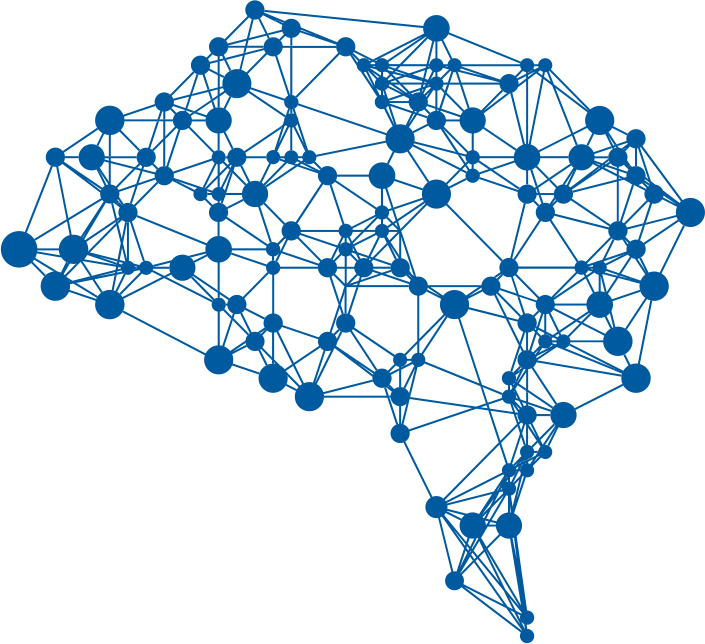
\includegraphics[width=0.8\textwidth]{deepLearning.png}\\
        \vspace{4cm}
        \normalsize{安捷 1601210097}\\
        \normalsize{\today}
    \end{titlepage}
        \section{算法实现简介}
            在这次作业中,我基于上一次作业实现的CNN模型,给CNN中添加了batch normalization层;同时,为了使得算法的代码更为清楚,我对上一次实现的代码进行了重构。
        \section{算法实现的函数功能简介}
            \begin{table}[htbp!]
                \centering
                \begin{tabular}{cc}
                    \hline
                    函数名称 & 功能 \\
                    \hline
                    conv\_2d & 卷积层线性单元 \\
                    max\_pool & 最大池化层 \\
                    
                    \hline
                \end{tabular}
                \caption{算法不同超参数下固定迭代次数达到的准确率}
            \end{table}
            从上表可以看出,不同的算法对于参数都有很大的敏感性,无论是学习率还是动量参数,都会影响最终的结果,比较显著的但是又不言自明的特点是,过小的参数会导致算法的收敛速度变慢,过大的参数会使得算法不收敛。
            \clearpage

    \section{代码运行环境及测试平台信息}
      \begin{table}[htbp!]
        \centering
        \begin{tabular}{l}
          \hline
          Python Version: 3.6.0 \\
          Tensorflow Version: tensorflow-gpu-1.0.1 \\
          CUDA Version: 8.0 \\
          OS: Arch Linux \\
          Kernel: x86\_64 Linux 4.10.4-1-ARCH \\
          CPU: Intel Core i7-6700K @ 8x 4.2GHz \\
          GPU: GeForce GTX 1060 6GB \\
          RAM: 16003MiB \\
          \hline
        \end{tabular}
        \caption{代码运行环境及测试环境表}
      \end{table}
      在没有NVIDIA\ GPU及CUDA支持的环境下代码依然可以运行,只是速度较慢
    \section{总结}
      通过这次作业,我学习了tensorflow实现cnn的基本方法,同时尝试使用了不同的优化算法来学习参数,发现了参数对算法结果的巨大影响,明白了调参的重要性。
\end{document}